\section{Problem Formulation}
In this section we present the general concept of our learning approach. The basic idea is to interpret the folded state of a box as a series of rotation angles along each edge, where the problem of predicting folded state is turned into a problem of predicting these angles. 
\subsection{Definitions and Notations}
As an input to our method, we expect a 2D designed layout of a box represented as a flat triangular mesh $L$. As output of our method, we deform the input triangular mesh into its 3D realization $R$, according to predicted angles along each of its edges.(An example is shown in Figure~\ref{fig:approximation})\\
\begin{figure}
	\centering
	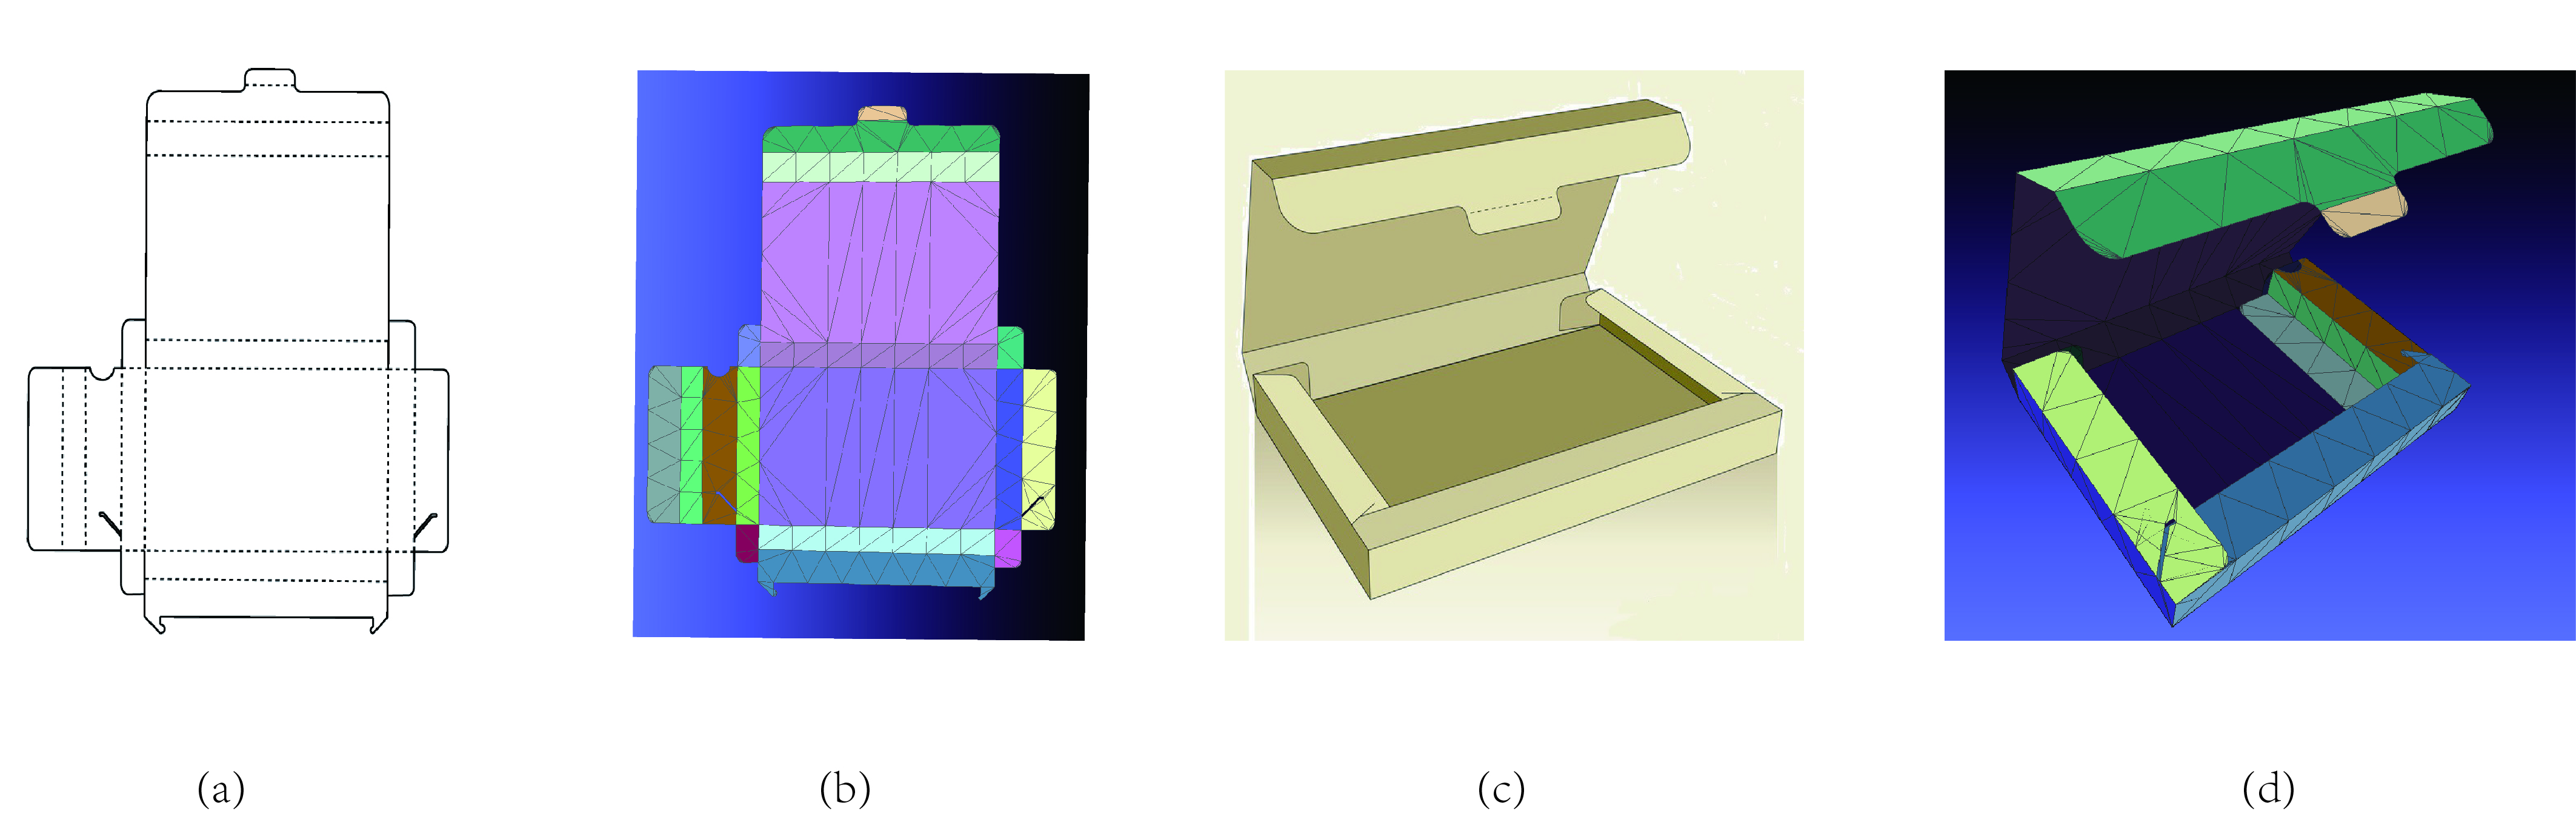
\includegraphics[width=3.0in]{images/approximation.jpg}
	\caption{Given a design layout (a) and its 3D realization (c), we can approximately represent them by triangular mesh as (b) and (d).}
	\label{fig:approximation}
\end{figure}
Without loss of generality, a learning approach should be able to learn an operator $F$ that maps every 2D layout to its 3D realization:
\begin{equation}
F:\{L\}\rightarrow\{R\}
\label{equ:F_0}
\end{equation}
in which $\{L\}$ is the set of all designed layout of boxes represented by 2D triangular meshes and $\{R\}$ is the set of 3D realization of the same boxes represented by deformed triangular meshes. For each triangular mesh 
\subsection{From Shape Mapping to Functional Mapping}
It is difficult to design a model and a learning scheme to learn the operator in (\ref{equ:F_0}).As we stressed before, the folded state of a box can be represented by a series of rotation angles along each edge.
\subsection{Choice of Features}
\subsection{Choice of Basis Functionals}
